\chapter{Motion-Aware Unitを用いた3波長を入力とした紫外線像の全球時系列予測}
  \section{実験概要}
    ここでは、171Å、193Åフィルターで得られたデータを追加で利用し、3波長の入力データから211Åの波長データに対する予測を行った。
    これらの波長は、太陽のコロナ領域における異なる温度帯を観測するためのものであり、予測モデルに多様な物理的情報を提供することが期待される。
    171Åの波長は、太陽のコロナにおける温度が約60万Kの領域を捉えるのに特化しており、193Åの波長は約100万Kの領域を捉える。
    これらの波長から得られる情報を組み合わせることにより、単一の波長では捉えられない層間の相互作用を捉え、より高い精度での予測を可能にすることを期待する。
    
    モデルには先の実験と同じく、MAUを用いる。入力は3波長、すなわち画像的には3チャンネルである。
    目的となる出力は211Åの波長のみであるが、MAUは3チャンネルを出力する。
    これは、「出力シークエンスのタイムステップ1以降では、直前のモデルの出力を入力データとして扱う」という動画予測モデルの一般的な性質によるものである。
    このような性質から、211Åの波長のみを出力として扱うために、出力された3チャンネルのうち、211Åの波長のみを抽出するという処理を行った。
  
  \section{実験設定}
    各ハイパーパラメータの設定を表\ref{tab:exp1_hyperparameters}に示す。チャンネル数のみ前回の実験から変更されている。
    \begin{table}[h]
      \centering
      \begin{tabular}{lc}
      \hline
      ハイパーパラメータ & 値 \\
      \hline\hline
      バッチサイズ & 4 \\
      \hline
      エポック数 & 100 \\
      \hline
      学習率 & 0.0005 \\
      \hline
      損失関数 & MSE \\
      \hline
      チャンネル & 3 \\
      \hline
      カーネルサイズ & (5, 5) \\
      \hline
      MAU Cell数 & 16 \\
      \hline
      \end{tabular}
      \caption{本実験でのハイパーパラメータ設定。基本的には前実験と同様であるが、チャンネル数が1から3に変更されている。}
      \label{tab:exp1_hyperparameters}
    \end{table}

    データに関しても、データ数の増減による影響がないように、前回の実験と同じ期間のデータを用いた。欠損期間なども同様である。

  \section{学習の推移}
  
  学習は図\ref{fig:exp2_learn_progress}のように推移した。学習の初期段階では、学習データに対する損失関数の値が急激に減少しているが、学習が進むにつれて収束に向かって緩やかに減少していることがわかる。
  また、学習損失、検証損失ともに、安定的に減少していることがわかる。
  学習にはNVIDIA RTX A6000を用い、完了までに約31時間を要した。
  \begin{figure}[htpb]
    \centering
    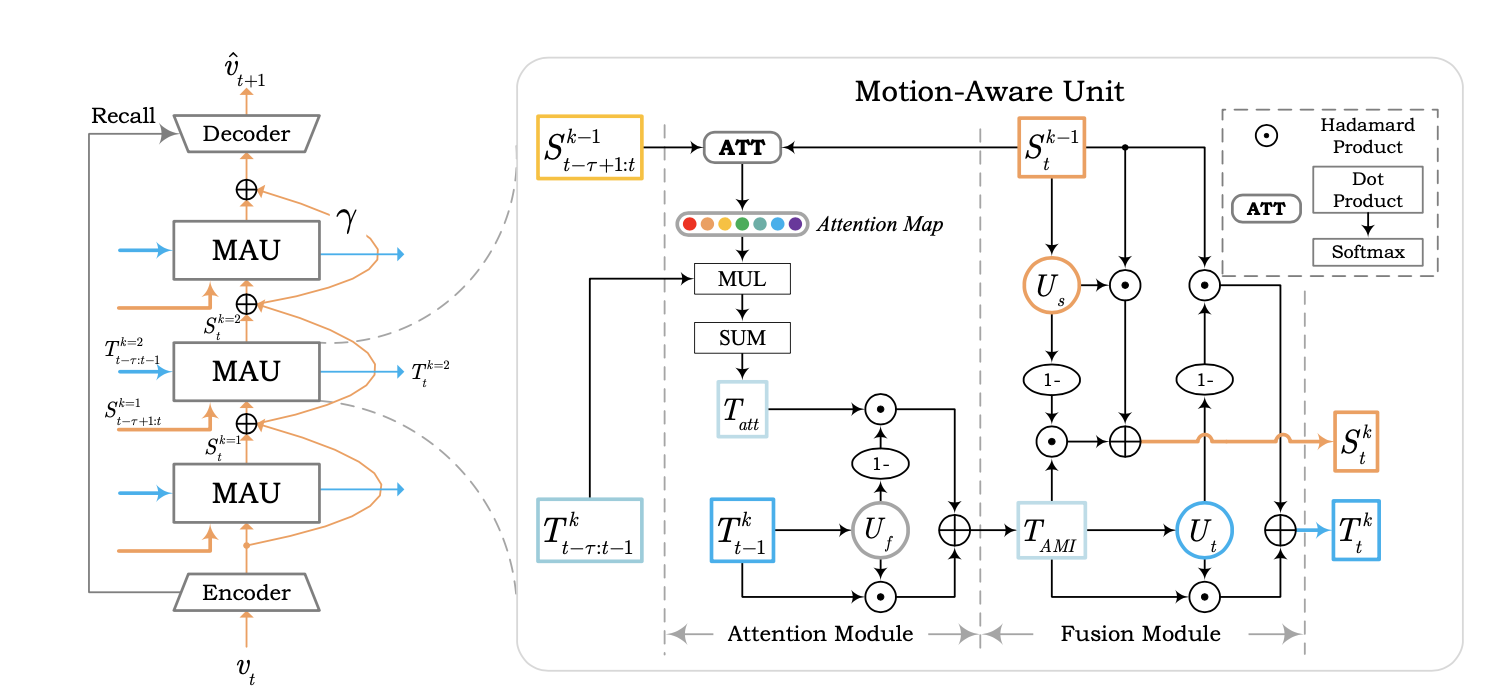
\includegraphics[width=\textwidth]{figures/mau.png}
    \caption{本実験での、学習データ、検証データでの損失関数の推移。どちらも安定的に減少している。}
    \label{fig:exp2_learn_progress}
  \end{figure}

  \section{実験結果}
    図\ref{fig:exp2_out}に、この実験での出力例を示す。
    \begin{figure}[h]
      \centering
      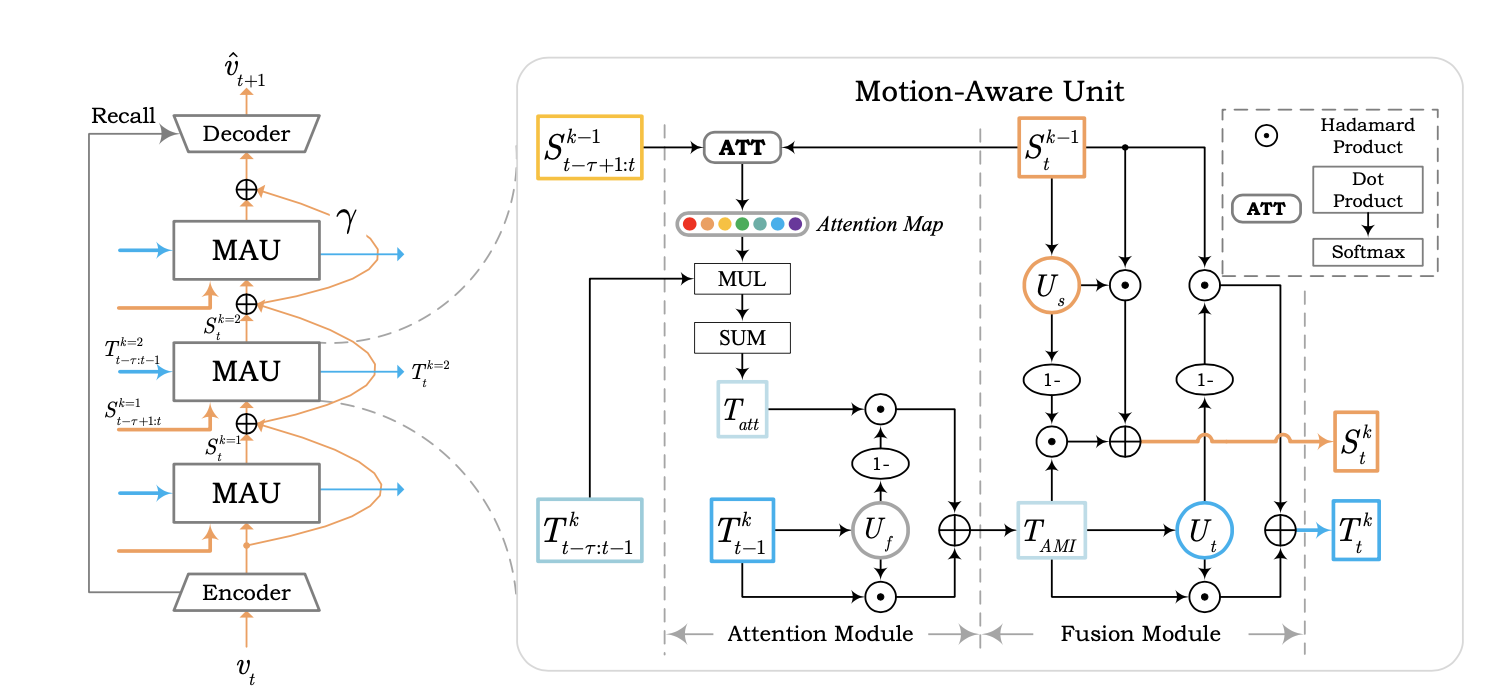
\includegraphics[width=\textwidth]{figures/mau.png}
      \caption{}
      \label{fig:exp2_out}
    \end{figure}
    モデルの出力は、視覚的には実際の観測画像と概ね合致している。
    この実験における評価では、前回の実験と同様の評価を行った。
  
    \subsection{全球での評価}
      はじめに全球での評価を行った。
      前回実験と同様に、まず輝度強度の平均値と実際の平均値との誤差、SSIMを計算した。さらに単純差動回転モデルとの比較も行った。
      また、これらの値の時間経過に対する変化を観察し、より不確定性の高い将来の予測に対しても動画予測モデルが有効であるかを検証した。

      \subsubsection{平均輝度とその誤差}
        モデルの出力の全球での平均輝度と、実際の観測画像との誤差の推移を図\ref{fig:exp2_mean_intensity_line}に示す。
        これは、50のテストセットに対して、各テストセットに含まれる各画像の全球での平均輝度を計算し、その時間ステップごとの平均値を取ったものである。

        \begin{figure}[h]
          \centering
          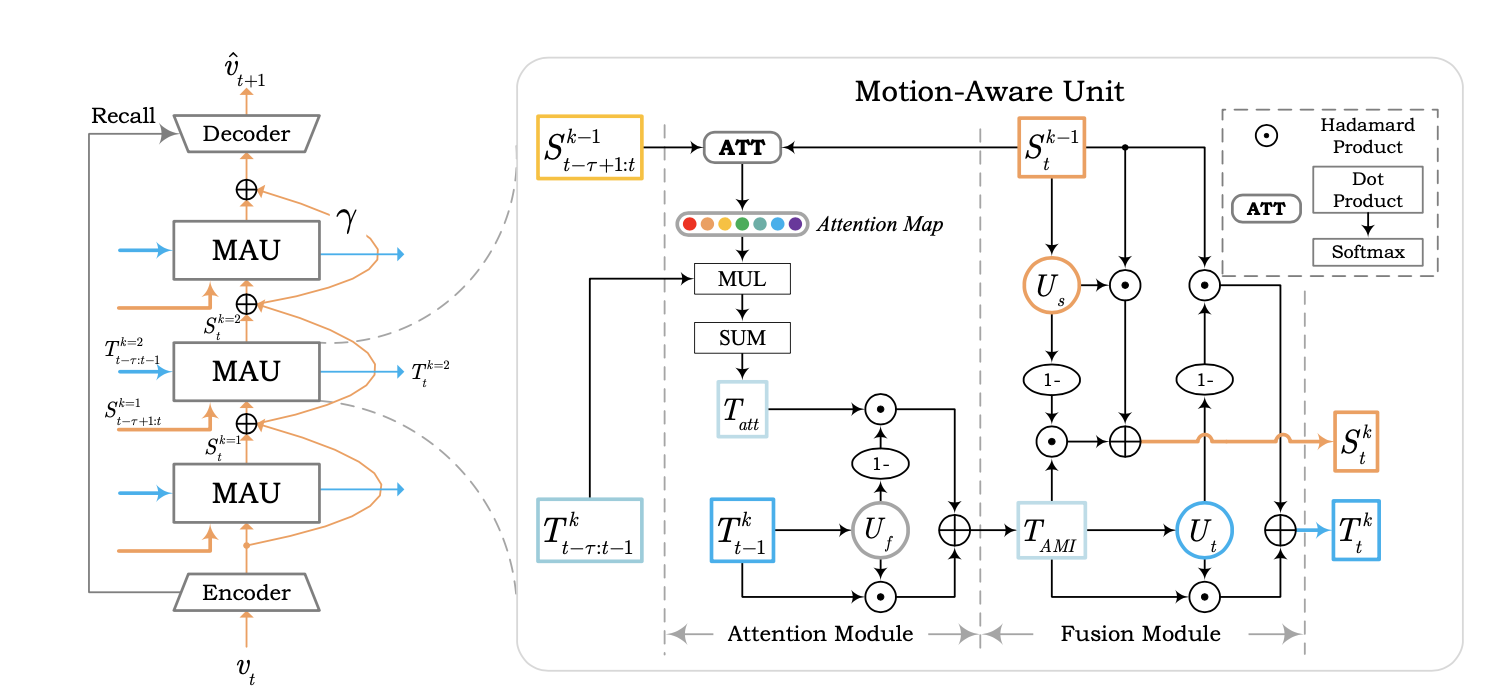
\includegraphics[width=\textwidth]{figures/mau.png}
          \caption{}
          \label{fig:exp2_mean_intensity_line}
        \end{figure}
        
        さらに、入力シークエンスの最後から48時間後の画像の全球での平均輝度と、実際の観測画像との差異を観察する。その散布図\ref{fig:exp2_mean_intensity_scatter}に示す。
        このタイムステップは、出力の最後のタイムステップであり、最も不確定性の高い予測である。

        \begin{figure}[h]
          \centering
          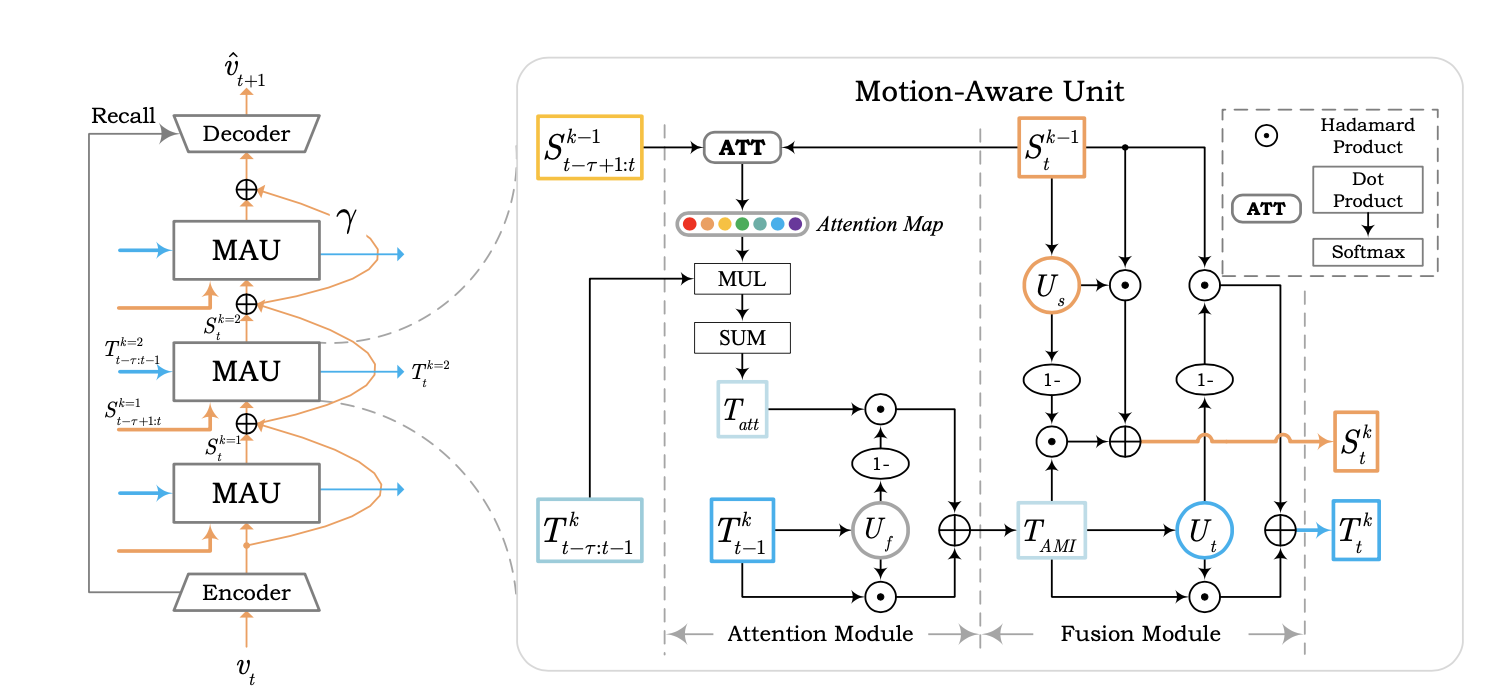
\includegraphics[width=\textwidth]{figures/mau.png}
          \caption{}
          \label{fig:exp2_mean_intensity_scatter}
        \end{figure}

      \subsubsection{画像類似度}
        前回実験と同様に、画像内での構造的再現度とその時間的変化を評価するために、モデルの出力と対応する時間ステップの実際の観測画像の間のSSIMを計算した。
        SSIMの推移を図\ref{fig:exp2_ssim_line}に示す。画像類似度は、全球での平均輝度と同様に、全球に対してのみ行い、画像中の背景や外縁部からはみ出すコロナなどはその計算に含まれない。
        \begin{figure}[h]
          \centering
          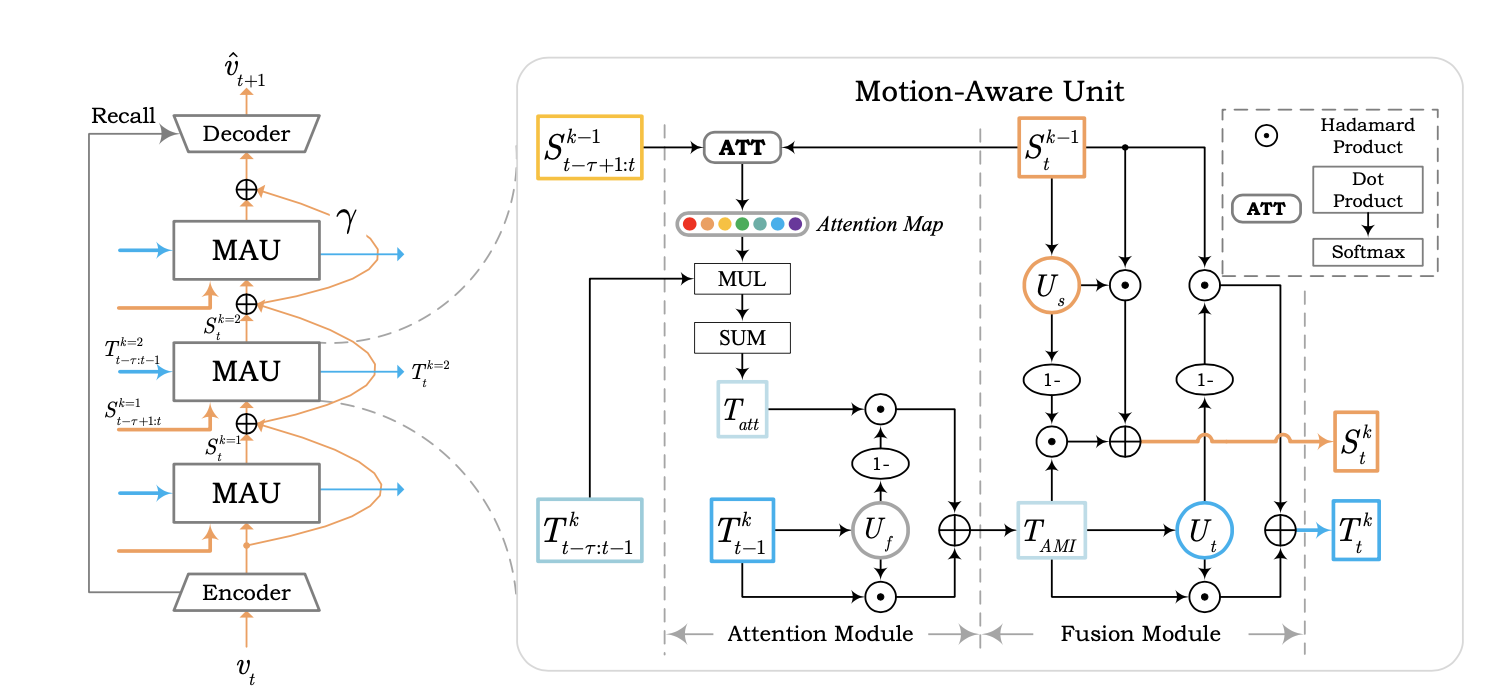
\includegraphics[width=\textwidth]{figures/mau.png}
          \caption{}
          \label{fig:exp2_ssim_line}
        \end{figure}

      \subsubsection{単純差動回転モデルとの比較}
        前回実験と同様に、モデルの予測性能をさらに詳細に評価するために、シンプルな差動回転モデルとの比較を行った。
        比較は、単純差動回転モデルによるシミュレーションと、実際の観測画像との間の平均輝度の絶対誤差を計算し、それを前述の動画予測によるものと比較することで行った。
        この誤差の推移を図\ref{fig:exp2_sdr_line}に示す。

        \begin{figure}[h]
          \centering
          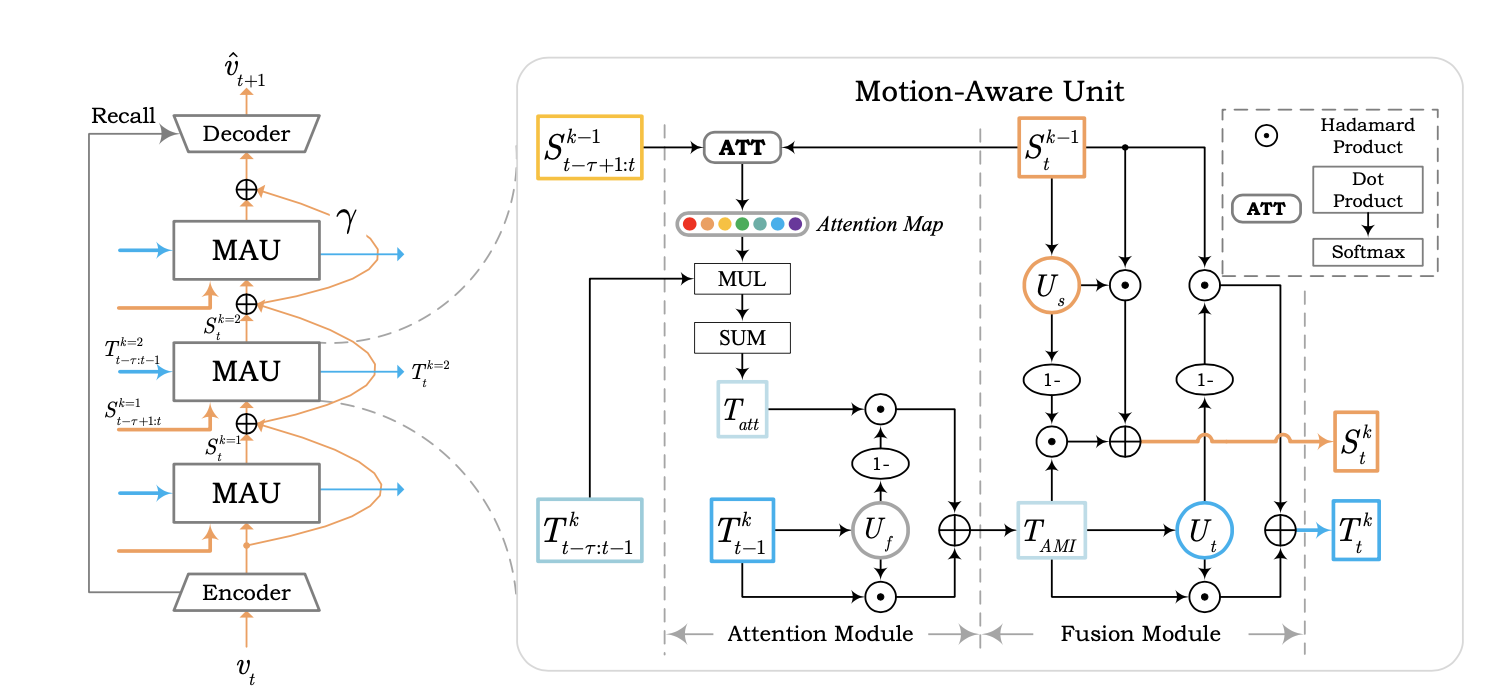
\includegraphics[width=\textwidth]{figures/mau.png}
          \caption{}
          \label{fig:exp2_sdr_line}
        \end{figure}
        
        さらに、出力シークエンスの最後のタイムステップにおいて、単純差動回転モデルによるシミュレーションと、実際の観測画像との差異を観察し、動画予測モデルによる出力と比較した。
        その散布図\ref{fig:exp2_sdr_scatter}に示す。
        
        \begin{figure}[h]
          \centering
          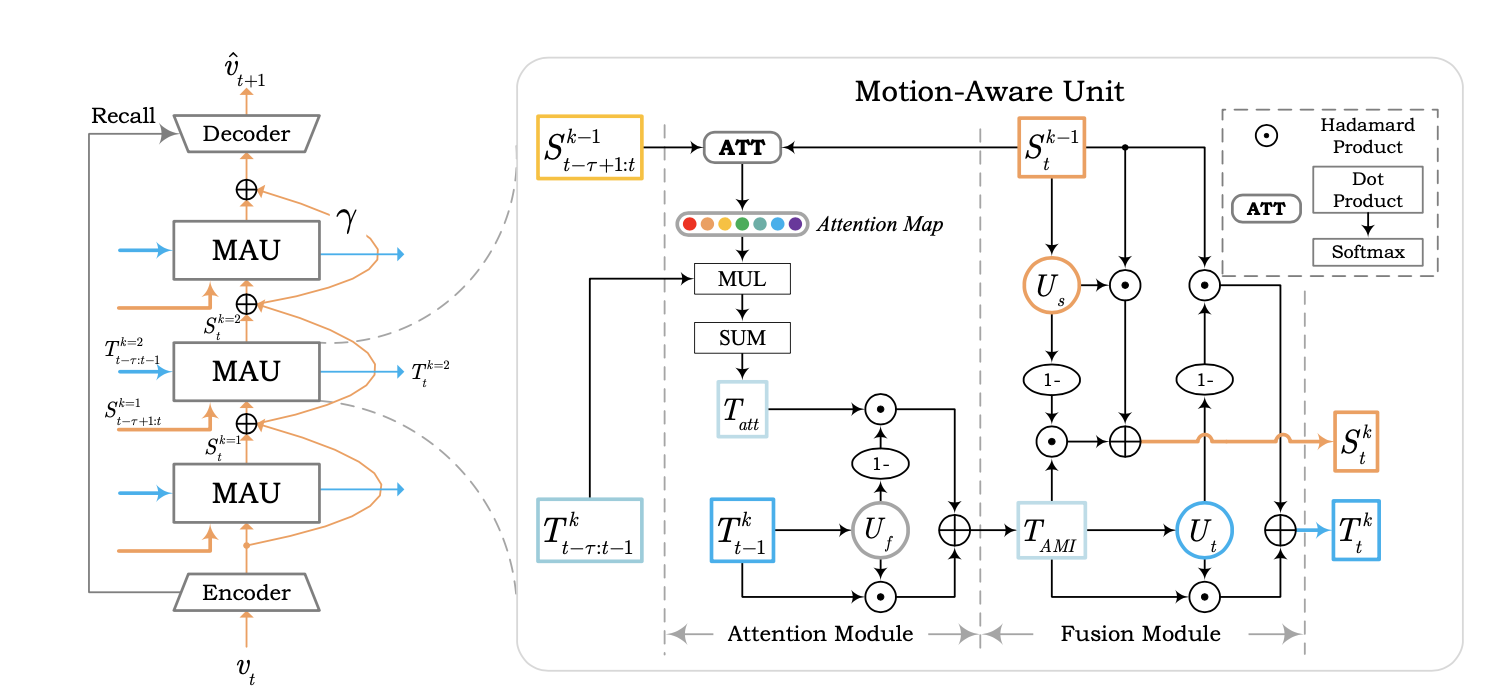
\includegraphics[width=\textwidth]{figures/mau.png}
          \caption{}
          \label{fig:exp2_sdr_scatter}
        \end{figure}
        
      \subsection{経度依存性の評価}
        前回実験と同じく、予測性能が経度ごとにばらつきがあるかを確認するために、経度ごと予測の再現度を評価した。分割の方法は前回実験と同様である。
        評価指標には、平均輝度の誤差と、その単純差動回転モデルとの比較を用いた。

        \subsubsection{平均輝度とその誤差}
          ここでは、全てのテストセットで各セクターごとの平均輝度を計算し、対応する時間ステップの実際の観測画像との間の絶対誤差を計算した。
          誤差率の時間推移を図\ref{fig:exp2_mean_intensity_longitude_line}に示す。
          \begin{figure}[h]
            \centering
            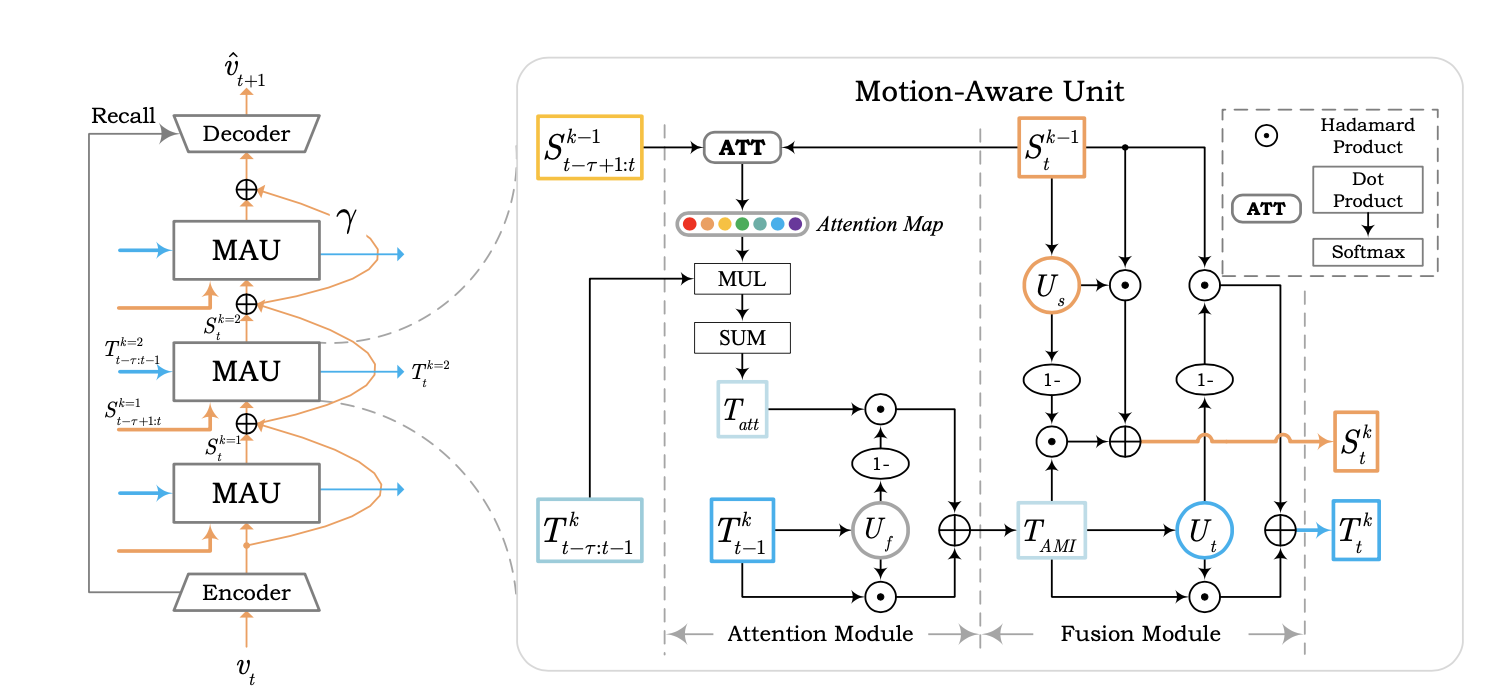
\includegraphics[width=\textwidth]{figures/mau.png}
            \caption{}
            \label{fig:exp2_mean_intensity_longitude_line}
          \end{figure}
          
          さらに、全球での評価と同様に、出力シークエンスの最後のタイムステップにおいて、動画予測モデルの出力から計算される経度ごとの平均輝度と、実際の観測画像での経度ごとの平均輝度をプロットした散布図を図\ref{fig:exp1_mean_intensity_longitude_scatter}に示す。
          
          \begin{figure}[h]
            \centering
            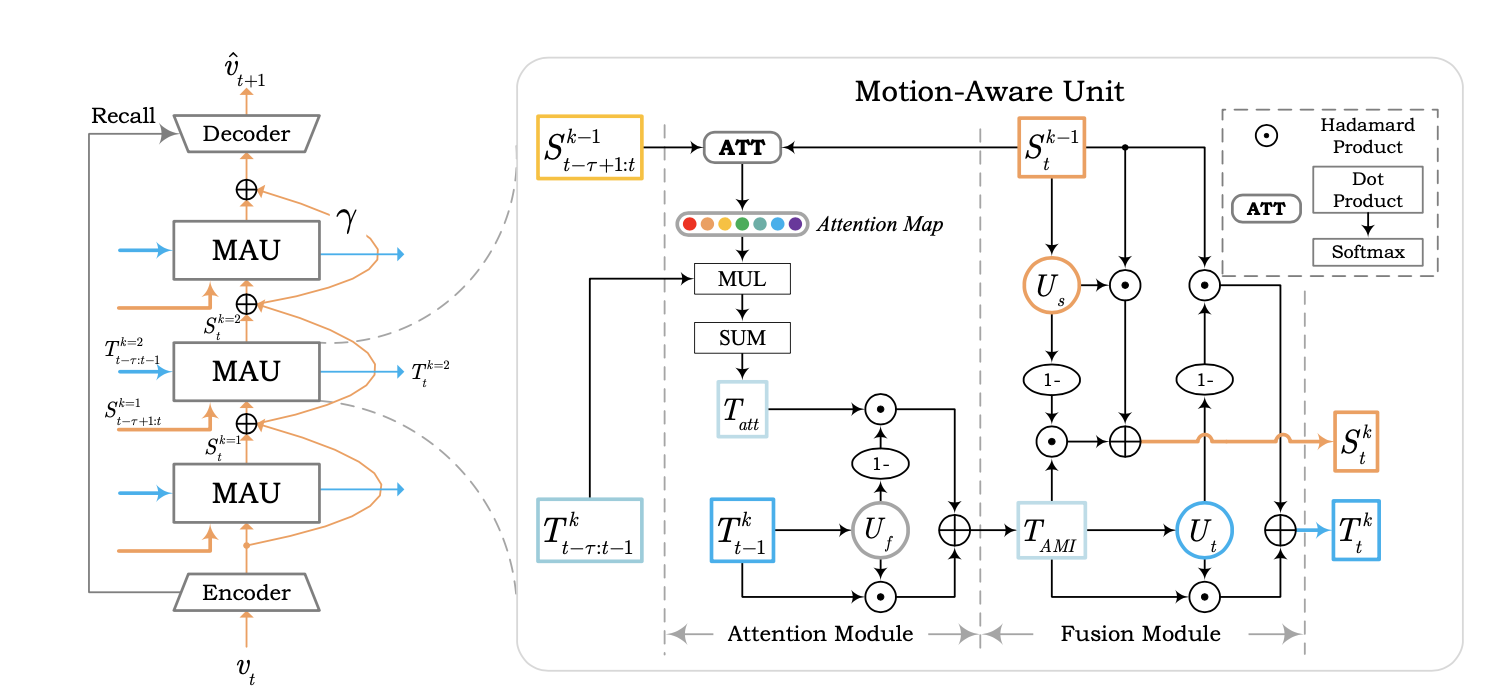
\includegraphics[width=\textwidth]{figures/mau.png}
            \caption{}
            \label{fig:exp2_mean_intensity_longitude_scatter}
          \end{figure}

        \subsubsection{単純差動回転モデルとの比較}
          全球での場合と同様に、経度ごとの比較でも単純差動回転モデルとの比較を行った。その時間推移を図\ref{fig:exp1_sdr_longitude_line}に示す。
          \begin{figure}[htbp]
            \centering
            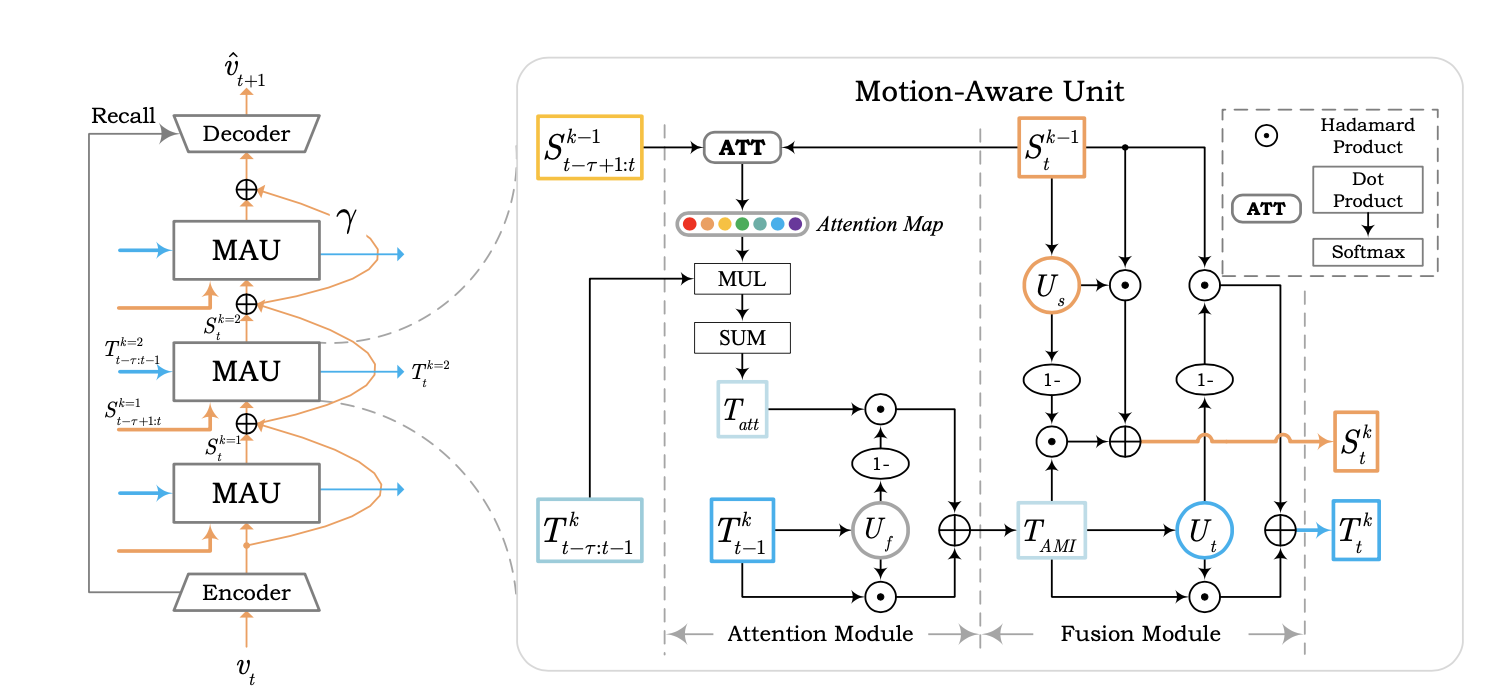
\includegraphics[width=\textwidth]{figures/mau.png}
            \caption{}
            \label{fig:exp1_sdr_longitude_line}
          \end{figure}
          
          また、出力シークエンスの最後のタイムステップにおける、経度ごとの単純差動回転モデルによるシミュレーションと、実際の観測画像との差異を観察し、動画予測モデルによる出力と比較した。
          その散布図を図\ref{fig:exp1_sdr_longitude_scatter}に示す。
          \begin{figure}[htbp]
            \centering
            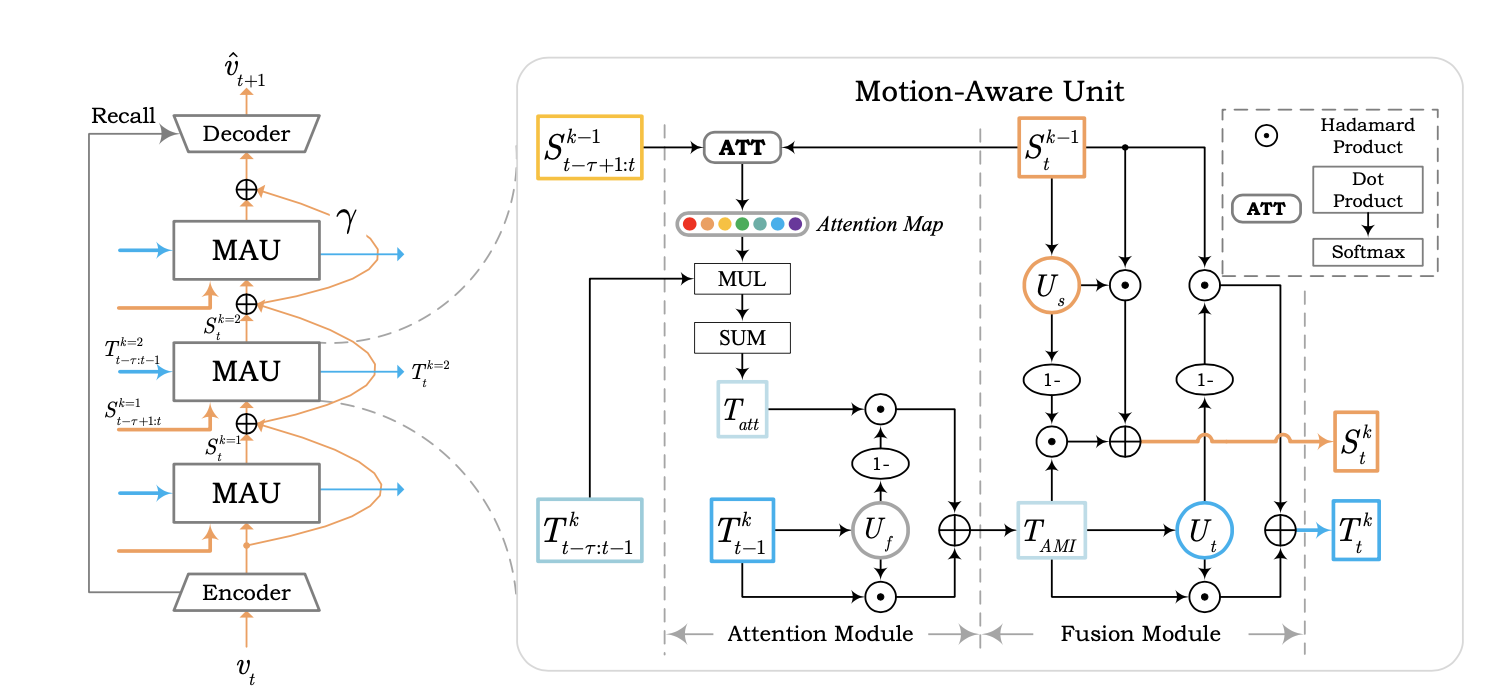
\includegraphics[width=\textwidth]{figures/mau.png}
            \caption{}
            \label{fig:exp1_sdr_longitude_scatter}
          \end{figure}

    \subsection{東側リムから出現する活動領域に対する視覚的評価}
  \section{考察}
